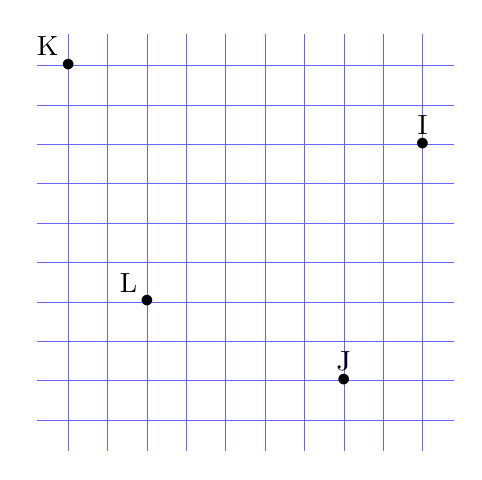
\begin{tikzpicture}	
  
    
\def \CharSize {1};
\def \BulletSize {1};


\draw[very thin, blue!60] (0.1,-0.9) grid[step=0.5] (5.4,4.4);

\draw (0.5,4) node [above left,scale=\CharSize]{K};
\draw (0.5,4) node[scale=\BulletSize]{$\bullet$};
\draw (1.5,1) node [above left,scale=\CharSize]{L};
\draw (1.5,1) node[scale=\BulletSize]{$\bullet$};
\draw (5,3) node [above,scale=\CharSize]{I};
\draw (5,3) node[scale=\BulletSize]{$\bullet$};
\draw (4,0) node [above,scale=\CharSize]{J};
\draw (4,0) node[scale=\BulletSize]{$\bullet$};
\end{tikzpicture} 